\documentclass[conference,letterpaper]{IEEEtran}

\usepackage{cite}
\usepackage{graphicx}
\usepackage{amsmath,amssymb}
\usepackage{algorithm}
\usepackage{algorithmic}
\usepackage{psfrag}

\IEEEoverridecommandlockouts

% AML bibliography references
\newcommand{\bib}[1]{/aml/home/mjg82/bib/#1}

% Better references, I think
\renewcommand{\sec}[1]{Section~\ref{sec:#1}}
\newcommand{\fig}[1]{Figure~\ref{fig:#1}}
\newcommand{\alg}[1]{Algorithm~\ref{alg:#1}}

% Algorithmic changes
\renewcommand{\algorithmicforall}{\textbf{for each}}

%% PSO Stuff
\DeclareMathOperator{\URand}{U}
\DeclareMathOperator*{\argmin}{arg\;min}
\DeclareMathOperator*{\argmax}{arg\;max}
\DeclareMathOperator*{\arginf}{arg\;inf}
\DeclareMathOperator*{\argsup}{arg\;sup}
\providecommand{\ppos}{\ensuremath{\Vec{x}}}
\providecommand{\pvel}{\ensuremath{\Vec{v}}}
\providecommand{\nbest}{\ensuremath{\Vec{b}_N}}
\providecommand{\pbest}{\ensuremath{\Vec{b}_P}}
\providecommand{\constriction}{\ensuremath{\chi}}
\providecommand{\coeff}{\ensuremath{\phi}}
\providecommand{\obs}{\ensuremath{\Vec{\xi}}}

%SpecExPSO Stuff
\providecommand{\noeval}[1]{\ensuremath{#1^{-e}}}
\providecommand{\nonbest}[1]{\ensuremath{#1^{-n}}}
\providecommand{\p}{\ensuremath{p}}
\providecommand{\pset}{\ensuremath{\mathbf{p}}}
\providecommand{\s}{\ensuremath{s}}
\providecommand{\sset}{\ensuremath{\mathbf{s}}}
\providecommand{\nsset}{\ensuremath{\mathbf{ns}}}
\providecommand{\n}{\ensuremath{n}}
\providecommand{\nset}{\ensuremath{\mathbf{n}}}
\providecommand{\nnset}{\ensuremath{\mathbf{nn}}}

\title{\ \\ \LARGE\bf Speculative Evaluation in Particle Swarm Optimization%
\thanks{Matthew Gardner, Andrew McNabb, and Kevin Seppi are with the Department
of Computer Science, Brigham Young University, 3361 TMCB, Provo, UT 84602
(phone: 801-422-8717; email: \{mjg82,a,k\}@cs.byu.edu).}%
}

\date{}

\author{Matthew Gardner, Andrew McNabb, and Kevin Seppi}

\begin{document}
\maketitle

\begin{abstract}

Particle swarm optimization (PSO) has previously been parallelized only by 
adding more particles to the swarm or by parallelizing the evaluation of the
objective function.  However, some functions are better optimized with more
iterations and fewer particles.  Accordingly, we take inspiration from 
speculative execution commonly performed in modern processors and propose what
we call speculative evaluation in PSO.  Future positions of the particles are
speculated and evaluated in parallel with current positions, performing two
iterations of PSO at once.

We also propose another way of making use of these speculative particles,
keeping the best position found instead of the position that PSO actually would
have taken.  We show results that for a number of functions, speculative
evaluation can have dramatic improvements over adding additional particles to
the swarm.

\end{abstract}

\section{Introduction}
\label{sec:intro}

Particle swarm optimization (PSO) has been found to be a highly robust and
effective algorithm for solving many types of optimization problems.  For much
of the algorithm's history, PSO was run serially on a single machine.  However,
the world's computing power is increasingly coming from large clusters of
processors.  Even in desktop machines, systems with 4 or 8 cores are
commonplace.  In order to efficiently utilize these resources for
computationally intensive problems, algorithms need to run in parallel.

Within the last few years, researchers have begun to recognize the need to
develop parallel implementations of PSO, publishing many papers on the subject.
The methods they have used include various synchronous algorithms
\cite{belal-ijicis04,chu-sci06,jin-aps05,parsopoulos-aia04,schutte-ijnme04},
asynchronous algorithms \cite{koh-ijnme06,mostaghim-report06,venter-wcsmo05},
and formulating PSO in Google's MapReduce framework \cite{mcnabb-cec07}.
Parallelizing the evaluation of the objective function can also be done in some
cases, though that is not an adaption of the PSO algorithm and thus is not the
focus of this paper.

All of these parallel techniques use additional processors to increase the
number of particles in the swarm, either by adding individual particles or by
adding entire new subswarms.  The number of iterations of PSO that the
algorithms can perform is thus inherently limited by the time it takes to
evaluate the objective function---additional processors add more particles, not
more iterations.  However, there are many functions for which performing more
iterations with fewer particles is a better use of resources than performing
fewer iterations with more particles.  

To solve this problem, we take inspiration from speculative execution
techniques commonly used in processors.  Modern processors, when faced with a
branch on which they must wait, guess which way the branch will go and start
executing.  If the processor guessed right, execution is much farther ahead
than if it had just idly waited on the branch.  If it guessed wrong, execution
restarts right where it would have been anyway.  This is called speculative
execution or branch prediction.

The idea of speculative execution can be applied to some types of optimization
algorithms.  When the next sampling position of the algorithm does not depend
explicitly on the value of the objective function at the current position,
future positions can be speculated and evaluated in parallel with the current
position.  This could not be done in gradient methods, for instance, where the
step size for sampling depends on the gradient at the current position, but it
has been done in simulated annealing~\cite{witte-tpds91}.

Because the motion of particles in PSO depends only on the \emph{positions} of
the particle and its neighbors, not the \emph{value} of the objective function
at those positions, speculative evaluation is possible.  We do not have to wait
for a particle's position to be evaluated to know where it might move to next,
so we can compute the set of all possible next positions and send them to be
evaluated along with the particle's current position.  Once the current
position of each particle has been evaluated, we can determine which of the
speculatively evaluated positions matches the branch taken by the particle.  We
have thus evaluated two iterations at once.  This can easily get unwieldy if
the set of next possible positions for each particle is large, but a wise
choice of topology limits that set to a reasonable size.

The original PSO can be reproduced exactly, two iterations at a time, using
this technique.  However, in strictly using speculative evaluation to reproduce
the original PSO, a lot of positions are speculatively evaluated whose values
get ignored after deciding which branch was the correct one.  A better use of
those speculative evaluations may be to incorporate the information into the
swarm, no longer exactly reproducing PSO but perhaps producing better results.

\sec{pso} describes the particle swarm optimization algorithm.  \sec{sepso}
then describes how speculative evaluation can be done in parallel PSO to
perform two iterations at once.  In \sec{extra}, we discuss a variant of the
speculative algorithm which uses all of the speculative evaluations performed
instead of throwing away all but one for each particle.  We then show in
\sec{results} a comparison between the original PSO algorithm, our speculative
algorithm, and its variant.  In \sec{conclusion} and \sec{future} we conclude
and discuss future work.

\section{Particle Swarm Optimization}
\label{sec:pso}

Particle swarm optimization was proposed in 1995 by James Kennedy and Russell
Eberhart~\cite{kennedy-icnn95}.  The algorithm is used to intelligently search
a multi-dimensional space by mimicking the swarming and flocking behavior of
birds and other animals. It is a social algorithm that depends on interaction
between particles to quickly and consistently find the optimal solution to some
objective function.

The motion of particles through the search space has three components: an
inertial component that gives particles momentum as they move, a cognitive
component where particles remember the best solution they have found and are
attracted back to that place, and a social component by which particles are
attracted to the best solution that any of their neighbors have found.

At each iteration of the algorithm, the position $\ppos_t$ and velocity
$\pvel_t$ of each particle are updated as follows:
\begin{align}
\label{eq:velupdate}
	\pvel_{t+1} &=
		\constriction \left[ \pvel_t +
			\coeff_1\URand()\otimes(\pbest - \ppos_t) +
			\coeff_2\URand()\otimes(\nbest - \ppos_t)
		\right] \\
\label{eq:posupdate}
	\ppos_{t+1} &= \ppos_t + \pvel_{t+1}
\end{align}
where \( \URand() \) is a vector of random numbers drawn from a uniform
distribution, the \( \otimes \) operator is an element-wise vector
multiplication, $\pbest$ (called personal best) is the best position the
current particle has seen, and $\nbest$ (called neighborhood best) is the best
position the neighbors of the current particle have seen.  \( \coeff_1 \), \(
\coeff_2 \), and \( \constriction \) are parameters with prescribed values
required to ensure convergence (2.05, 2.05, and .73,
respectively)~\cite{clerc-tec02}.

There are many ways of defining the neighbors of a particle.  Different
neighborhood topologies have varying performance on different kinds of
functions, as would be expected by the No Free Lunch
theorem~\cite{wolpert-tec97}.  An in-depth discussion of topologies in PSO is
beyond the scope of this paper.  The two most common topologies used in the
literature are the Ring topology and the Complete
topology~\cite{bratton-sis07}.  In this paper we use those topologies, as well
as a parallel adaptation of the Complete topology called Random that has been
shown to simulate the behavior of Complete with far less
communication~\cite{mcnabb-cec09}.  Both the Ring and the Random topologies can
be defined as having $k$ neighbors; we use 2 neighbors for all of our
experiments.

\section{Speculative Evaluation in PSO}
\label{sec:sepso}
\subsection{Overview}

The PSO algorithm just described can be parallelized by having each additional
processor add a particle or a set of particles to the swarm.  But for some
functions, a more desirable use of resources is to speed up the algorithm,
performing more iterations instead of adding more particles.  Barring
parallelizing the evaluation of the objective function itself, which may not be
possible, previous techniques have not addressed this issue.

In order to perform additional iterations by adding additional processors, we
take inspiration from speculative execution in processors.  If we can guess
what a particle's next position will be from its current position, we can
evaluate both in parallel and perform two iterations of PSO at once.  Lacking
a good way to guess a particle's next position, we can at least enumerate all
possible next positions of the particle, evaluate all of them at once, and one
of them will be right.

While in some algorithms enumerating all possible next sampling positions would
be impossible or extremely difficult, in PSO all we need to know are the
current positions of the particle and its neighbors, from which we can easily
enumerate and evaluate all possible positions of that particle at the next
iteration.  The defining components of a particle's motion
(see~\eqref{eq:velupdate}) are $\pvel_t$, $\ppos_t$, $\pbest$, and $\nbest$.
For a particle at iteration $t-1$, $\pvel_t$ and $\ppos_t$ are defined by
Equations~\eqref{eq:velupdate} and \eqref{eq:posupdate}.  The only remaining
components are $\pbest$ and $\nbest$, each of which has only a few
possibilities.  The particle already knows its personal best $\pbest$ at
iteration $t-1$, but it could be updated to $\ppos_t$ if its position at
iteration $t$ has a better value than its current personal best.  Likewise, the
particle knows its neighborhood best $\nbest$ at iteration $t-1$, though it
could be updated by any of its neighbors' positions at iteration $t$.

To enumerate all of the possible next positions of a particle, one must simply
evaluate the motion equations for all possible combinations of personal best
and neighborhood best updates that a particle could see.  This produces
$2(n+1)$ speculative positions to be evaluated, where $n$ is the number of
neighbors the particle has.  If a particle is also its own neighbor, as is most
often the case, one of the $2(n+1)$ speculative positions can be eliminated, as
a particle cannot be the source of its $\nbest$ update while not updating its
$\pbest$.  Table~\ref{tab:evals} lists all possible combinations of updates
that can be seen by a particle with two neighbors other than itself, which is
the case in all of the topologies we use.  If all of these speculative
positions are evaluated in parallel along with the original, non-speculative
position of the particle at time $t-1$, then one of the speculative positions
has to be the correct one, and two iterations have been evaluated at once.

\begin{table}
  \caption{All possible updates for a particle with two neighbors}
  \label{tab:evals}
  \centering
  \begin{tabular}{c|c}
	$\pbest$ updated&Source of $\nbest$ update\\
	\hline
	No update&No update\\
	Updated&No update\\
	No update&Neighbor 1\\
	No update&Neighbor 2\\
	Updated&The particle itself\\
	Updated&Neigbhor 1\\
	Updated&Neighbor 2\\
  \end{tabular}
\end{table}

Because $2(n+1)$ speculative evaluations must be performed for each particle,
the choice of topology is an important one.  The use of the Complete topology,
where every particle is a neighbor to every other particle, would require on
the order of $p^2$ speculative evaluations per iteration, where $p$ is the
swarm size.  Clearly it is much more desirable to have a sparse topology, where
$O(np)$ is much smaller than $O(p^2)$.  However, some functions are better
optimized with the Complete topology and the quick spread of information it
entails than with sparse topologies.  Accordingly, we use the Random topology
described in~\cite{mcnabb-cec09}, which has been shown to effectively simulate
the Complete topology.  In that topology, 2 neighbors are chosen at random from
the swarm for each particle at each iteration.  Because a particle is also
always its own neighbor, $n$ is $3$ in that case.  In~\sec{results} we report
the results for performing speculative evaluation using both the Ring topology
(where $n$ again is $3$) and the Random topology on a number of common
benchmark functions.

It is not trivial in some parallel architectures to determine which speculative
position was the correct next position of each particle.  First we discuss the
relatively easy case of a centralized parallel PSO algorithm.  In such an
architecture, the master keeps track of all necessary information with only
trivial message passing needed.  Then we discuss the more complicated case of a
distributed algorithm, where each particle is on its own and needs to send and
receive messages to and from other particles.  Finally we discuss the further
complications of a dynamic topology, where a particle's neighbors change from
one iteration to another.

\subsection{Terminology}

To aid in describing our methodology, we introduce a few terms.  A particle's
set of \emph{speculative children} is the set of all possible next iteration
states that a particle could have.  We use $\p_t$ to denote a particle at
iteration $t$ and $\s_{t+1}$ to denote one of $\p_t$'s speculative children,
corresponding to one of the rows in Table~\ref{tab:evals}.  $\n_t$ is a
neighbor of particle $\p_t$.  A set of particles is $\pset$, $\sset$, or
$\nset$, whereas a single particle is simply $\p$, $\s$, or $\n$.

We separate each iteration of PSO into several steps.  First there is the
motion step, where a particle updates its position and velocity.  Then a
particle's position is evaluated, and the particle updates its current value
and its personal best.  Finally, a particle gets information from its neighbors
and updates its neighborhood best.

A particle at iteration $t-1$ that has been moved to iteration $t$, but whose
position has not yet been evaluated, is denoted as $\noeval{\p}_t$.  Once its
position has been evaluated, but it has still not yet received information from
its neighbors, it is denoted as $\nonbest{\p}_t$.  Only when the particle has
updated its neighborhood best is it a complete particle at iteration $t$.  It is
then simply denoted as $\p_t$.

\subsection{Centralized Algorithms}

\begin{algorithm}
  \caption{Speculative Evaluation in a Centralized PSO}
  \label{alg:centralized}
  \begin{algorithmic}[1]
	\STATE Move all $\p_{t-1}$ to $\noeval{\p}_t$
	\STATE For each $\noeval{\p}_t$, get its neighbors $\noeval{\nset}_t$ and
	  generate $\noeval{\sset}_{t+1}$
	\STATE Evaluate all $\noeval{\p}_t$ and $\noeval{\sset}_{t+1}$ in parallel
	\STATE Update personal best for each $\noeval{\p}_t$ and
	  $\noeval{\s}_{t+1}$, creating $\nonbest{\p}_t$ and $\nonbest{\s}_{t+1}$
	\STATE Update neighborhood best for each $\nonbest{\p}_t$, creating
	  $\pset_t$
	\FORALL{$\p_t$}
	\STATE Pick $\nonbest{\s}_{t+1}$ from $\nonbest{\sset}_{t+1}$ that matches
	  the branch taken by $\p_t$
	\STATE Pass along personal and neighborhood best values obtained by $\p_t$,
	  making $\nonbest{\p}_{t+1}$
	\ENDFOR
	\STATE Update neighborhood best for each $\nonbest{\p}_{t+1}$, creating
	  $\pset_{t+1}$
	\STATE Repeat
  \end{algorithmic}
\end{algorithm}

In a centralized, or Master-Slave, parallel PSO algorithm, one machine, the
master, keeps track of all necessary information, and all other machines are
merely used to evaluate the objective function at various positions as directed
by the master~\cite{belal-ijicis04}.  To perform speculative evaluation in such
a scheme, the master generates the positions to evaluate speculatively and
decides which one to accept for each particle.

Given a set of particles at iteration $t-1$ (perhaps which have just been
initialized), the master must move each particle using
Equations~\eqref{eq:velupdate} and \eqref{eq:posupdate} to obtain the set
$\noeval{\pset}_t$.  For each particle $\noeval{\p}_t$, the master must get its
set of neighbors $\noeval{\nset}_t$ and use their positions, along with the
position of $\noeval{\p}_t$, to enumerate all possible combinations of $\pbest$
and $\nbest$ that particle $\noeval{\p}_t$ could end up with (as shown in
Table~\ref{tab:evals}).  Each of those combinations defines a speculative
particle, $\s_t$, that can be moved using the motion equations to obtain
$\noeval{\s}_{t+1}$.  The result is a set of particles $\noeval{\pset}_t$, and
for each particle a set of speculative children $\noeval{\sset}_{t+1}$, which
can all be evaluated at once.

The master then has the slaves evaluate the particles.  Once all particles,
speculative and original, have been evaluated and the values reported to the
master, the master sorts out which speculative child of each particle was the
correct one.

This is done by first updating each particle $\noeval{\p}_t$ to
$\nonbest{\p}_t$ and each speculative particle $\noeval{\s}_{t+1}$ to
$\nonbest{\s}_{t+1}$ by associating the value determined by the slave to the
particle it came from, and updating that particle's personal best if the value
reported is better than its previous personal best value.  Then each
$\nonbest{\p}_t$ must be updated to $\p_t$ by updating its neighborhood best
position and value with information about each of its neighbors.  This is
simply the original PSO algorithm.

Then, with the set $\pset_t$, the branch that was actually taken by each
particle can be determined, and the correct speculative child can be chosen.
The branches depend entirely on whether or not the personal best of $p_t$ was
updated and which particle, if any, updated the particle's neighborhood best.
Both of those items are now known, and the child that matches the branch is
selected.

The parent $\p_t$ must pass its personal best value to the child, as the child
knows only the position that it guessed, not the function value at that
position.  It is possible that both $\p_t$ and $\s_{t+1}$ update their
personal bests, but $\p_t$'s value is better.  For example, suppose that
$\p_{t-1}$ has a personal best value of 3.  $\noeval{\p}_t$ is created, and
$\noeval{\s}_{t+1}$ is moved assuming that $\p_t$ has updated its personal
best with its position at time $t$.  Then both $\noeval{\p}_t$ and
$\noeval{\s}_{t+1}$ are evaluated, with values 1 and 2, respectively.
$\nonbest{\s}_{t+1}$ would think that its current position is its personal
best, as the value it found, 2, is better than its previous personal best
value of 3.  It needs to receive the personal best value from its parent to
know that its personal best position $\pbest$ is actually the position of
$\p_t$, not $\s_{t+1}$.

The parent also needs to pass the value of the neighborhood best that the child
guessed.  The child only knows the position and needs the value in order to
make future comparisons between neighborhood best positions.

Upon picking the correct branch for each particle and updating the children's
personal best and neighborhood best value (from iteration $t$), the result is
the set $\nonbest{\pset}_{t+1}$, as the particles are now no longer
speculative.  What remains is to update the neighborhood best of those
particles from their neighbors (from iteration $t+1$), as above, to obtain
$\pset_{t+1}$.  That set of particles can subsequently be used to produce the
sets $\noeval{\pset}_{t+2}$ and $\noeval{\sset}_{t+3}$, and the process repeats
itself.

The algorithm is outlined in \alg{centralized}.

\subsection{Distributed Algorithms}

In a distributed parallel PSO algorithm, individual processors not only perform
evaluations of particles, but also their movement.  The information for each
particle is not held by a central machine that directs the algorithm; instead,
each processor has the information for the particle or particles that it is in
charge of and must perform the steps of the algorithm for those particles.
Messages such as values and positions for the neighborhood best are sent
between processors.  There may be some machine that collects information from
all of the particles and outputs the result of the algorithm, though that
machine's importance is much less than in centralized algorithms.

To perform speculative evaluation in a distributed PSO algorithm, there must be
some way to have processors evaluate the speculative children of particles,
without giving the speculative particles the same treatment as actual
particles, as the speculative children only live for one iteration.  Perhaps
that can be done by assigning each particle a set of machines instead of a
single machine, and the particle directs its extra machines to evaluate its
speculative children.  No matter the distributed framework used the message
passing should be similar, and that is what we describe here.

A processor that is controlling a single particle $\p_{t-1}$ must first move
the particle to $\noeval{\p}_t$ and produce the particle's speculative children
$\noeval{\sset}_{t+1}$.  This is done in the same way as described above.
However, in order to produce $\noeval{\sset}_{t+1}$, the processor needs
information about the particle's neighbors, so there must be some message
passing to get that information.  Particularly, the information that the
processor needs is the position of each of the particle's neighbors at
iteration $t$.

To get that information, a round of message passing is required.  Each particle
sends its position to its neighbors at iteration $t$, so that all particles can
generate $\noeval{\sset}_{t+1}$.  After each particle evaluates its position
and the positions of its speculative children, it passes information about the
outcome of iteration $t$ to its neighbors, so that neighboring particles can
update their neighborhood bests to move from $\nonbest{\p}_t$ to $\p_t$.  Once
that communication is finished, the particle can select the speculative child
which matched the branch that iteration $t$ actually produced.  Then another
round of information passing follows, for iteration $t+1$, so that
$\nonbest{\p}_{t+1}$ can be updated to $\p_{t+1}$.  Two iterations have then
been completed with only one round of evaluations, and the next iteration can
start again with the first round of message passing.

\subsection{Alternate form of message passing}

In some distributed frameworks, like the MapReduce framework that we used in
our experiments, rounds of message passing can be expensive.  The method
just described uses three rounds of message passing for every two iterations.
Accordingly, we describe a method that requires only one round of communication
for each pair of iterations.  A lot more messages are needed, but that is
sometimes more desirable than synchronizing all of the machines three times.

This second method only requires one round of passing information because
information about iterations $t$ and $t+1$ is passed at the same time.  Each
processor reconstructs from the messages it receives all of the information
that it needs about its neighbors.  Messages are passed directly after
evaluating each particle and its children, so all messages are of the form of
$\nonbest{\p}_t$ or $\nonbest{\s}_{t+1}$.  The first iteration needs to be
treated specially, so each particle can produce its initial set of speculative
children---neighbors need only pass their initial position.  This kind of
message passing necessitates the careful use of random seeds, so that when each
processor computes the motion equations for its neighbors it gets the same
results as its neighboring processors.

With the results of evaluating $\noeval{\p}_t$ and $\noeval{\sset}_{t+1}$,
along with all of the required messages from neighboring particles, the goal is
to produce $\p_{t+1}$ and output $\noeval{\p}_{t+2}$ and $\noeval{\sset}_{t+3}$
ready to be evaluated for the next iteration.  We first focus on the messages
needed to produce $\p_{t+1}$.

Upon evaluation, $\noeval{\p}_t$ becomes $\nonbest{\p}_t$, needing only to get
its neighborhood best information from its neighbors.  All of its neighbors,
then, must send it a message, so that from their updated personal best at
iteration $t$ the particle becomes $\p_t$.  The work done with the messages
received thus far is just as in regular PSO, and is graphically depicted in 
\fig{messages1}.

\begin{figure}
  \centering
  \psfrag{pt-n}[C][C]{$\nonbest{\p}_{t}$}
  \psfrag{nt-n}[C][C]{$\nonbest{\nset}_{t}$}
  \psfrag{pt}[C][C]{$\p_{t}$}
  \includegraphics[width=.3\columnwidth]{messages1.eps}
  \caption{The messages needed to produce $\p_{t}$.  Items without an arrow
  pointing to them are messages the particle needs to receive.}
  \label{fig:messages1}
\end{figure}

With $\p_t$ we can select the correct speculative child as described above and
produce $\nonbest{\p}_{t+1}$.  Again we show the use of messages thus far
graphically, in \fig{messages2}.  

\begin{figure}
  \centering
  \psfrag{pt-n}[C][C]{$\nonbest{\p}_{t}$}
  \psfrag{nt-n}[C][C]{$\nonbest{\nset}_{t}$}
  \psfrag{pt}[C][C]{$\p_{t}$}
  \psfrag{pt1-n}[C][C]{$\nonbest{\p}_{t+1}$}
  \psfrag{st1-n}[C][C]{$\nonbest{\sset}_{t+1}$}
  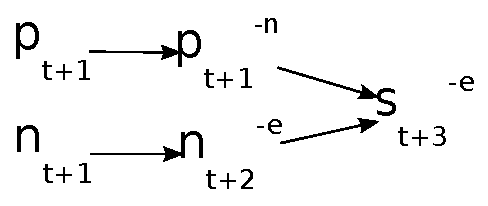
\includegraphics[width=.5\columnwidth]{messages2.eps}
  \caption{The messages needed to produce $\nonbest{\p}_{t+1}$.  Items without
  an arrow pointing to them are messages the particle needs to receive.}
  \label{fig:messages2}
\end{figure}

We then need the set of neighbors to $\nonbest{\p}_{t+1}$,
$\nonbest{\nset}_{t+1}$, so we can update $\nonbest{\p}_{t+1}$'s neighborhood
best.  To produce each neighbor $\nonbest{\n}_{t+1}$, we need the same
information for the neighboring particle that we needed to produce the original
particle, $\nonbest{\p}_{t+1}$; we need the original neighbor particle, its
speculative children, and its neighbors.  With that information, the set
$\nonbest{\nset}_{t+1}$ can be obtained by following the same process used to
obtain $\nonbest{\p}_{t+1}$.  We graphically show the messages needed to
produce $\nonbest{\nset}_{t+1}$ in \fig{messages3}.  Note that it looks
identical to \fig{messages2}, just with different sets of particles.

\begin{figure}
  \centering
  \psfrag{nt-n}[C][C]{$\nonbest{\nset}_{t}$}
  \psfrag{nnt-n}[C][C]{$\nonbest{\nnset}_{t}$}
  \psfrag{nt}[C][C]{$\nset_{t}$}
  \psfrag{nt1-n}[C][C]{$\nonbest{\nset}_{t+1}$}
  \psfrag{nst1-n}[C][C]{$\nonbest{\nsset}_{t+1}$}
  \includegraphics[width=.6\columnwidth]{messages3.eps}
  \caption{The messages needed to produce $\nonbest{\nset}_{t+1}$.  Items
  without an arrow pointing to them are messages the particle needs to receive.
  $\nnset$ is the set of neighbors for each particle $\n$, and $\nsset$ is the
  set of $\n$'s speculative children.  Note the similarity between this and
  \fig{messages2}.}
  \label{fig:messages3}
\end{figure}

With $\nonbest{\nset}_{t+1}$ and $\nonbest{\p}_{t+1}$, we can produce
$\p_{t+1}$.  This is shown in \fig{messages4}.  Note that we just combined
Figures~\ref{fig:messages2}~and~\ref{fig:messages3}, putting them together
to make $\p_{t+1}$, as all the particle needs is it's neighborhood best to be
updated.

\begin{figure}
  \centering
  \psfrag{pt-n}[C][C]{$\nonbest{\p}_{t}$}
  \psfrag{nt-n}[C][C]{$\nonbest{\nset}_{t}$}
  \psfrag{pt}[C][C]{$\p_{t}$}
  \psfrag{pt1-n}[C][C]{$\nonbest{\p}_{t+1}$}
  \psfrag{st1-n}[C][C]{$\nonbest{\sset}_{t+1}$}
  \psfrag{nt-n}[C][C]{$\nonbest{\nset}_{t}$}
  \psfrag{nnt-n}[C][C]{$\nonbest{\nnset}_{t}$}
  \psfrag{nt}[C][C]{$\nset_{t}$}
  \psfrag{nt1-n}[C][C]{$\nonbest{\nset}_{t+1}$}
  \psfrag{nst1-n}[C][C]{$\nonbest{\nsset}_{t+1}$}
  \psfrag{pt1}[C][C]{$\p_{t+1}$}
  \includegraphics[width=.8\columnwidth]{messages4.eps}
  \caption{The messages needed to produce $\p_{t+1}$.  Items
  without an arrow pointing to them are messages the particle needs to receive.
  Note that this is just a combination of \fig{messages2} and \fig{messages3}.}
  \label{fig:messages4}
\end{figure}

In order to get $\p_{t+1}$, then, a particle needs to receive messages from its
neighbors, its neighbors' neighbors, its speculative children, and its
neighbors' speculative children.  The particle $\p_{t+1}$ can be passed to some
central machine to track the progress of the algorithm, and it can be moved to
$\noeval{\p}_{t+2}$ in order to start the next iteration.

The next goal is to produce the set $\noeval{\sset}_{t+3}$.  As described
above, the necessary components to produce $\noeval{\sset}_{t+3}$ are
$\noeval{\p}_{t+2}$ and the neighbors of $\noeval{\p}_{t+2}$,
$\noeval{\nset}_{t+2}$.  We already have $\noeval{\p}_{t+2}$, so what remains
is to produce $\noeval{\nset}_{t+2}$.  It is sufficient to obtain
$\nset_{t+1}$, as each neighbor particle $\n_{t+1}$ can be moved with the
motion equations to $\noeval{\n}_{t+2}$.

We have already described how to use a set of messages to obtain $\p_{t+1}$.
The process is exactly the same to produce each $\n_{t+1}$, requiring the same
messages, except for the neighbor particles instead of the particle itself.  
\fig{messages5} shows graphically how $\noeval{\sset}_{t+3}$ is produced.

\begin{figure}
  \centering
  \psfrag{pt1}[C][C]{$\p_{t+1}$}
  \psfrag{nt1}[C][C]{$\nset_{t+1}$}
  \psfrag{nt2-e}[C][C]{$\noeval{\nset}_{t+2}$}
  \psfrag{pt2-e}[C][C]{$\noeval{\p}_{t+2}$}
  \psfrag{st3-e}[C][C]{$\noeval{\sset}_{t+3}$}
  \includegraphics[width=.5\columnwidth]{messages5.eps}
  \caption{The messages needed to produce $\noeval{\sset}_{t+3}$. $\p_{t+1}$
  and $\nset_{t+1}$ are both produced as in \fig{messages4}.}
  \label{fig:messages5}
\end{figure}

Having obtained both $\noeval{\p}_{t+2}$ and $\noeval{\sset}_{t+3}$ from the
messages received, the algorithm then moves to the evaluation phase, and the
process repeats itself.  The particles are evaluated, send their messages, and
produce the next set of particles to be evaluated from the messages received.

To perform the entire process, at each message passing round a particle must
receive messages from its neighbors, its neighbors' neighbors, its neighbors'
neighbors' neighbors, its speculative children, its neighbors' speculative
children, and its neighbors' neighbors' speculative children.  With the Ring
topology, that looks like more messages than it really is, as many of the
neighbors' neighbors are duplicates.  With the Random topology, however, the
list of necessary messages could be rather large.  

This may seem like an inordinate amount of work, and in some instances it is.
However, some parallel frameworks necessitate this type of message passing, so
we have described how speculative evaluation can be performed in such
frameworks.

\subsection{Dynamic Topologies}

Performing speculative evaluation in PSO with a dynamic topology raises a few
issues of its own.  First, with neighbors changing each iteration, messages
that processors pass to their neighbors need to be sent to the correct
neighbors for each iteration.  In centralized algorithms and in distributed
algorithms with several rounds of message passing (the first method described
above), nothing needs to be changed.  However, in the case where processors
reconstruct information about neighboring particles from messages, those
messages need to be sent to the correct neighbors.  A particle cannot simply
send messages to its neighbors' neighbors' neighbors---it needs to send
messages to its iteration $t$ neighbors' iteration $t+1$ neighbors, and so on.
For every neighbor outward information is sent, the iteration also needs to be
incremented, as information about neighbors' neighbors is used during iteration
$t+1$, and information about neighbors' neighbors' neighbors is used to
reconstruct information about iteration $t+2$.  Also, this method of message
passing again requires the use of random seeds if the topology is random.

Also, an issue common to all methods of performing speculative evaluation is
that of getting available information from neighbors before generating
speculative children.  In a static topology, at iteration $t$ a particle
already has all of the information about the positions of its neighbors during
iterations $1$ through $t-1$.  If the neighbor finds a better position at 
iteration $t$, the particle updates its neighborhood best, but if it does not,
it still has its old neighborhood best from its neighbors for all previous 
iterations.

In a dynamic topology, a particle might not have information about the previous
positions of its neighbors at iteration $t$.  That means that its new
neighborhood best could come not only from its neighbors' positions at
iteration $t$, but also from their personal best from iteration $t-1$, as
neighbors' personal bests are what are used to update a particle's neighborhood
best.  That creates a problem for speculative evaluation---there are
potentially more than $2(n+1)$ possible next positions, increasing the amount
of work that must be done to perform the second iteration at the same time as
the first.

This is easily fixed by updating $\noeval{\p}_{t+2}$ with the currently
available information about $\noeval{\nset}_{t+2}$ before producing
$\noeval{\sset}_{t+3}$.  If a particle $\noeval{\p}_{t+2}$ updates its 
neighborhood best with the personal bests of $\noeval{\nset}_{t+2}$ before
calculating the next possible positions for $\noeval{\sset}_{t+3}$, there are
still only $2(n+1)$ possible next positions, and the problem is avoided.

\section{Using All Speculative Evaluations}
\label{sec:extra}

In performing speculative evaluation as we have described it, $2(n+1)$
speculative evaluations are done per particle, while all but one of them are
completely ignored.  It seems reasonable to try to make use of those
evaluations instead of throwing them away.  Making use of them changes the
behavior of PSO, instead of reproducing it exactly as the above method
explains, but the change could be an improvement.

To use the extra speculative evaluations, instead of choosing the speculative
child that matches that branch that the original PSO would have taken, we take
the child that has the best value.  The methodology is exactly the same as
above except for the process of choosing which speculative child to accept.
The branch that PSO would have taken is ignored, but $\p_t$ must still be
created so it can give the right personal best and neighborhood best values and
positions to $\p_{t+1}$.  The only change needed in \alg{centralized} is in
step 7, where the $\noeval{\s}_{t+1}$ with the best value is chosen from
$\noeval{\sset}_{t+1}$ instead of with the matching branch.

This can be thought of as drawing a number of samples from the next iteration
and accepting the best one.  Speculative particles that move in good directions
are kept.  It seems this modification to PSO would produce more exploitation,
decreasing the amount of exploration.  With functions that are less deceptive
we would expect this method to work well, while performance on more deceptive
functions would probably be hurt.

\section{Results}
\label{sec:results}

In our experiments we compared our speculative PSO algorithm to the standard
PSO algorithm.  To use the same number of processors for each algorithm,
speculative evaluation needs a smaller swarm size than standard PSO.  For each
of the topologies we used, a particle has two neighbors other than itself.  As
shown in Table~\ref{tab:evals}, this results in $7$ speculative evaluations per
particle.  With one evaluation needed for the original, non-speculative
particle, we have $8p_s$ evaluations for every two iterations, where $p_s$ is
the number of particles in the speculative swarm.  The extra evaluations done
in speculative evaluation would instead be particles in regular PSO, so we
compare swarms of size $p_s$ in speculative evaluation with swarms of size
$8p_s$ in regular PSO.

We use a Random topology in our speculative algorithm, as the Complete topology
leads to an explosion of speculative evaluations.  However, if speculative
evaluation were not being performed, it is likely that the Complete topology
would be used, ignoring the communication cost of Complete over Random.  To be
fair in our comparisons, for the standard PSO algorithm we compare to both the
Random topology with two neighbors and to the Complete topology.  All functions
have 20 dimensions, and all results shown are averages over 20 runs.  We use
240 processors in our experiments, so speculative algorithms use 30 particles
and standard PSO uses 240 particles.  For ease of labeling, we call our
speculative algorithm SEPSO, the variant SEPSO Pick Best, and standard PSO just
PSO.

First we look at the function Sphere, the simplest of common benchmark
functions.  Its equation is $f(\Vec{x}) = \sum_{i=1}^D x_i^2$.  The function
has no local optima and is best optimized in terms of function evaluations with
a small swarm using a Complete topology.  Accordingly, we show results for a
small Complete swarm in \fig{sphere1}.  In comparing SEPSO with PSO, we can see
that SEPSO clearly beats PSO with a Random topology.  However, the performance
between SEPSO and PSO Complete is not as encouraging---PSO Complete performs
slightly better.  But SEPSO Pick Best handily outperforms all other algorithms
in this problem.

\begin{figure}
  \centering
  \includegraphics[width=.8\columnwidth]{sphere1.eps}
  \caption{Function Sphere with a swarm that uses 240 processors per round of
  evaluations.  Speculative algorithms have a swarm of 30 particles and do two
  iterations per round, while standard PSO algorithms use 240 processors and do
  one iteration per round.}
  \label{fig:sphere1}
\end{figure}

Next we look at the function Griewank, defined by the equation $f(\Vec{x}) =
\frac{1}{4000} \sum_{i=1}^D x_i^2 - \Pi_{i=1}^D \cos\left(\frac{x_i}{\sqrt{i}}
\right) + 1$.  It is generally recommended to use the Ring topology when
optimizing the Griewank function, as Complete is prone to premature convergence
on a local optima.  We show results in \fig{griewank1} for swarms of size 30
and 240 using the Ring topology. One can see in the figure that both SEPSO
algorithms initially outperformed PSO, but got stuck in a local optima and were
eventually outperformed themselves.  

\begin{figure}
  \centering
  \includegraphics[width=.8\columnwidth]{griewank1.eps}
  \caption{Function Griewank with a swarm that uses 240 processors per round of
  evaluations.  Speculative algorithms have a swarm of 30 particles and do two
  iterations per round, while standard PSO algorithms use 240 processors and do
  one iteration per round.}
  \label{fig:griewank1}
\end{figure}

\fig{griewank1} is slightly deceptive, however, as with Griewank some of the
runs found the global optimum, 0, while some did not.  A more accurate plot for
this function is one showing what percentage of the runs have found the global
optimum at each iteration.  \fig{griewank2} shows such a plot.  A swarm of size
30 performing the PSO algorithm gets stuck a little less than half of the time,
while 240 particles provides enough exploration to find the global optimum
every time.  Surprisingly, using the SEPSO Pick Best algorithm with 30
particles greatly improves the chance of success with Griewank, while also
finding the global optimum in far fewer rounds of evaluations than standard
PSO.

\begin{figure}
  \centering
  \includegraphics[width=.8\columnwidth]{griewank2.eps}
  \caption{Function Griewank with a swarm that uses 240 processors per round of
  evaluations.  Instead of showing average function value, we show the
  percentage of runs that have found the global optimum by each iteration.}
  \label{fig:griewank2}
\end{figure}

Lastly we look at a function that does not show much or any improvement with
this method.  The function Rastrigin is defined as $f(\Vec{x}) = \sum_{i=1}^D
\left(x_i^2 - 10\cos\left(2\pi x_i\right) + 10\right)$.  It has been shown that
with Rastrigin, the more particles there are in the swarm, the lower function
value it finds, up to at least 4000 particles~\cite{mcnabb-cec09}.  Smaller
swarms get caught in local optima.  Because our speculative algorithms have a
significantly smaller swarm size, they get stuck at higher values while the
larger swarms performing regular PSO continue to improve the best value found.
\fig{rastrigin} shows the results graphically.

\begin{figure}
  \centering
  \includegraphics[width=.8\columnwidth]{rastrigin.eps}
  \caption{Function Rastrigin with a swarm that uses 240 processors per round
  of evaluations.  Speculative algorithms have a swarm of 30 particles and do
  two iterations per round, while standard PSO algorithms use 240 processors
  and do one iteration per round.}
  \label{fig:rastrigin}
\end{figure}

\section{Conclusions}
\label{sec:conclusion}

We have described how parallel implementations of particle swarm optimization
can be modified to allow additional processors to increase the number of
iterations of the algorithm performed, instead of merely adding more particles
to the swarm.  We have detailed several different implementations of the
algorithm, depending on the parallel PSO framework being used.  Using our
modifications, the original PSO algorithm is exactly reproduced two iterations
at a time.  This technique requires more function evaluations per iteration
than regular PSO, but for some functions still performs better when run in a
parallel environment.

We have also described a method for making use of extra speculative evaluations
that performs incredibly well on some functions.

Though space has limited our presentation of results to a very small sample of
the interesting and relevant applications of our technique, we believe the
results shown are sufficient motivation for the further exploration of
speculative evaluation in PSO.

Our results show that performing speculative evaluation instead of increasing
swarm size is only beneficial for some functions at the swarm sizes we used.
However, we would venture that for all functions there is some point at which
increasing the swarm size provides relatively little benefit.  At that point,
additional processors should be used to speed up the algorithm instead of add
additional particles.

There are some functions for which almost no exploration needs to be done;
Sphere is an example of such a function, as would be a function where the
general area of the optimal point is known, but the exact point needs to be
found.  For such functions the best use of processors is to have a small swarm
performing speculative evaluation with our second method, where all speculative
evaluations are used.

There are other functions for which there is a point where the algorithm has
done ``enough'' exploration and consistently finds the global optimum.  Adding
additional particles to the swarm is akin to increasing its capacity for
exploration.  We have seen that for a 20-dimensional Griewank function, a
number of particles greater than 30 but less than 240 has ``enough''
exploration and finds the optimal value every time.  For these functions, one
should use processors to increase the swarm size until enough exploration has
been reached, then use additional processors to increase the number of
iterations performed.

There are still other functions for which it seems there is never enough
exploration, such as the Rastrigin function.  It has been shown that up to 4000
particles there is no point at which ``enough'' exploration has been
done~\cite{mcnabb-cec09}.  For those functions the correct use of processors
cannot be easily prescribed and depends largely on the desired outcome.  It is
likely that the best thing to do with those functions is to use all processors
to add particles to the swarm and do no speculative evaluation.

\section{Future Work}
\label{sec:future}

This work represents the first attempt of which we are aware at using
additional processors in parallel with PSO to do something other than either
add particles to the swarm or parallelize the evaluation of the objective
function.  We anticipate that many future advancements can be made.  For
example, our technique required speculatively evaluating every possible next
position of each particle.  The number of speculative evaluations could
potentially be greatly reduced by using statistics for which branch of motion
particles most often follow.  Only the subset of the most probable next
locations would then be evaluated.  Using an asynchronous PSO variant may also
be helpful in this case, allowing particles to be at different iterations in
case the correct branch was not guessed and needs to be evaluated separately.

Another possible advancement would be to reduce communication costs by dropping
some of the inter-processor messages in distributed frameworks.  The PSO
algorithm would have to be adapted to work with less information, perhaps not
requiring that each processor have completely accurate information about what
neighboring particles are doing.

Still another possibility is to view the set of possible evaluations as an
infinite tree.  Each level in the tree is an iteration, and the branches on
each level represent the possible next positions of the particle.  One need not
simply evaluate all of one level for each particle---perhaps going two or three
iterations ahead on the most likely path would perform better.

We have mentioned that this technique has been previously used to parallelize
simulated annealing.  Any other optimization algorithm that only depends on 
current sampling positions when computing the next position to sample can be
parallelized with this technique.  In particular, genetic algorithms produce
future generations by combining individuals from the current generation.  With
a large population size there would be an unwieldy amount of possible future
individuals, but the potential exists to modify the algorithm to use some kind
of speculative evaluation.  A related but quite distinct technique for reducing
computation in evolutionary algorithms was proposed in~\cite{poli-ai06}.

Large parallel clusters are often required to successfully optimize practical
modern problems.  To properly use PSO with such clusters, a balance needs to be
made between using processors to increase the swarm size and using them to
increase the speed of the algorithm, or for perhaps as yet unconsidered
techniques.  This work is a first step in that direction.

\bibliographystyle{unsrt}
\bibliography{%
\bib{wolpert-tec97},%
\bib{merris-01},%
\bib{pso/clerc-tec02},%
\bib{pso/kennedy-icnn95},%
\bib{pso/bratton-sis07},%
\bib{pso/largeswarms/perez-emc05},%
\bib{pso/largeswarms/montes-gecco08.bib},%
\bib{pso/topology/liang-sis05.bib},%
\bib{pso/parallel/belal-ijicis04},%
\bib{pso/parallel/chu-sci06},%
\bib{pso/parallel/jin-aps05},%
\bib{pso/parallel/koh-ijnme06},%
\bib{pso/parallel/mostaghim-report06},%
\bib{pso/parallel/parsopoulos-aia04},%
\bib{pso/parallel/schutte-ijnme04},%
\bib{pso/parallel/venter-wcsmo05},%
\bib{ga/poli-ai06},%
\bib{sim-anneal/parallel/witte-tpds91.bib},%
\bib{pso/topology/kennedy-cec02.bib},%
\bib{pso/topology/mohais-cec04.bib},%
\bib{pso/topology/jordan-gecco08.bib},%
\bib{pso/topology/clerc-oep03.bib},%
\bib{pso/topology/miranda-ijcir08.bib},%
\bib{pso/topology/mendes-phd04.bib},%
\bib{aml/mcnabb-cec07},%
\bib{aml/mcnabb-cec09}}

\end{document}
